%!TEX root = ../dissertation.tex

\chapter{Background}
\label{chapter:background}
Your chapter's content goes here.

%Identify relevant concepts and technologies.
%- Web technologies(HTTP, HTML, CSS, Javascript, node.js, WebGL)
%- UI: event driven programming
%- 3D modeling for architecture
%- Programming in architecture / Generative Design

%Learnable Programming? (programming user interfaces)

%Identify relevant related work. Describe what they are, what they do, why are they relevant to our goals. Explain pros and cons / differences to our solution or goals.
%Programming environments? ("IDE for GD" no projecto de tese)
%- Rosetta: "one API, multiple languages and CADs"
%- Impromptu
%- IPython
%- Processing
%- DesignScript
%Programming environments a usar tecnologias web? ("Moving to the Web" no projecto de tese)
%- LightTable
%- OpenJSCAD
%- (IPython)
%Comparison + Problems to address
%% Others?
%- Grasshopper
%- Dynamo
%- Generative Components
%- Clara.io
%- OnShape
%% Discuss IDE features?
%- Rosetta traceability?
%- Program analysis: AST, instrumentation
%% Discuss predefined primitives?



%%Relevant to my work
%- Web applications - converted + new
%- 3D modeling tools - manual + programmatic
%- 3D modeling tools - primitives
%- Programming tools


%% Bruno Ferreira - Rosetta Revit BIM
% How it works? / Features
% The good aspects
% The bad aspects
% [Why it matters for the thesis?]
%%


%##############################################################################
%##############################################################################
\section{Related Work}


\subsection{Impromptu}
\label{section:impromptu:related}
Impromptu\cite{sorensen2005impromptu,sorensen2010programming} is a programming environment developed to explore manipulation of musical structure in live performance; an \gls{ide} for musicians and sound artists.

%What is live-performance?
Using Impromptu, live performance takes place as a musician programs algorithms that produce music in front of an audience.
During his performance, he writes the program that produces the sounds and chooses the right moments to change it to move between different parts of the music.

%What does it provide to support live-performance?
To enable live programming Impromptu brings together four components: an audio synthesizer, a real-time scheduling engine, a Scheme interpreter and an \gls{ide}.
The first three components make up the runtime environment, responsible for producing the sound, while the last provides an user interface, where the musician writes programs and sends them to the runtime.

%Describe live programming experience of impromptu.
As he sends code, the musician builds the algorithm that produces the music incrementally.%
\footnote{The code sent to the runtime can define/redefine functions or variables, and schedule audio or functions to be played or run later.}
To be able to keep producing sound for the audience he can program simple patterns, send them to the runtime and then change them as he programs more elements to compose the music.
As he adds more elements he can start to make small changes to some of them which will be immediately audible.

The immediacy from program changes to audible ones also lets the musician experiment with new ideas.
Similarly, someone doing \gls{gd} will also benefit from having this immediacy in his \gls{ide}.


\subsection{IPython}
\label{section:ipython:related}
IPython\cite{PER-GRA:2007} is a notepad-like environment (Fig. \ref{fig:ipython:notebook}) directed towards providing better, more straightforward, scientific computing.

As its name suggests, IPython's main programming language is Python.
Nevertheless, other popular programming languages can be used in IPython, particularly those popular in the scientific community like R, or Julia.%
\footnote{More language kernels can be found in IPython's github page: https://github.com/ipython/ipython/wiki/IPython-kernels-for-other-languages}

One trend in its community, one that is supported by IPython notebooks, is to make results in publications more reproducible.
Instead of publishing a PDF or making a blog post, authors write whole publications as IPython notebooks which then are shared and thus allow everyone to run their source code.
Having access to a working copy of the notebook, one can also experiment with it to better understand it, form own conclusions, and find potential errors.

%IPython architecture
IPython was decomposed into execution kernels, a communication protocol, and several front-ends.
As each type of component has a defined interface it is possible to implement new specialized components (a new front-end or a new execution kernel) that will integrate with those already implemented.

\begin{figure}
	\centering
	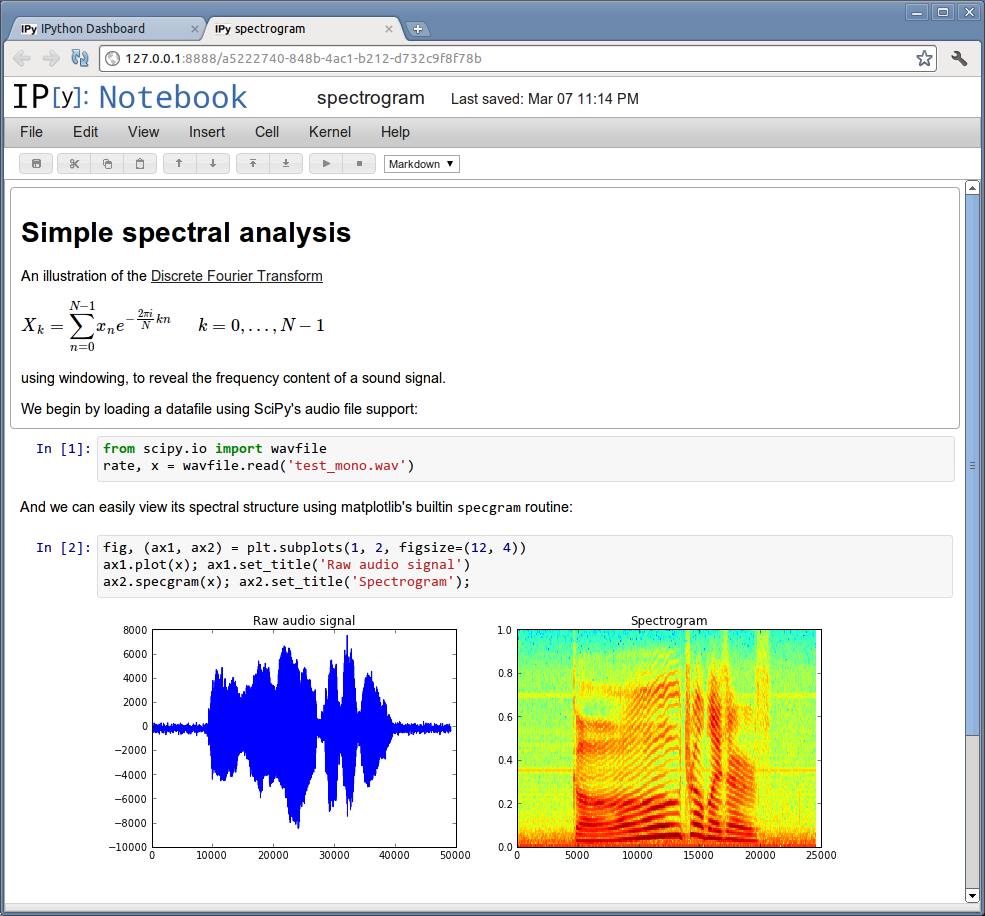
\includegraphics[width=0.8\textwidth]{images/ipython_notebook}
	\caption{An IPython notebook with rich text, mathematical notation, source code and results from executing such code.}
	\label{fig:ipython:notebook}
\end{figure}

%Why is it important? I cannot imagine designers using it.
As seen in Figure~\ref{fig:ipython:notebook}, IPython's notebooks can contain not only source code but also its results and rich text.
The style of producing notebooks in IPython is one that mixes programming, writing and exploring.
Interestingly, this style is also part of a designer's processes.
Like a scientist, the designer also has to do exploration of ideas (design ideas in his case), reach conclusions (finished designs) and share his work with others (fellow designers, clients, friends, blog readers).
Unfortunately, although IPython notebooks are natural tools for exploration, they do not provide domain specific functionality for architecture.


\subsection{Processing}
\label{section:processing:related}
Processing\cite{reas2007processing} is a programming language and a development environment aimed at ``promoting software literacy in the visual arts and visual literacy within technology''.\footnote{Quoting www.processing.org, 9/Nov/2015.}

Processing enables everyone to write programs that both draw to the screen and react to input from the user, like moving the mouse or pressing a key on the keyboard.
It makes this possible by implementing most of the functionality that is commonly required, like initializing the drawing surface, so the programmer only has to implement the functionality specific to the result he wants to achieve.
The code in Listing \ref{lst:simple:processing}, for instance, is what is needed to setup a drawing canvas, its background color and continuously draw a line from the mouse position to a point on the canvas.

To use Processing's programming language, one needs to use its \gls{ide}, the \acrfull{pde}.
As shown in Fig. \ref{fig:proc:dev:env}, the \gls{pde} includes a text editor with syntax highlighting and runs Processing programs.

\begin{listing}
	\begin{minted}[linenos]{java}
	//Hello mouse.
	void setup() {
		size(400, 400);
		stroke(255);
		background(192, 64, 0);
	}

	void draw() {
		line(150, 25, mouseX, mouseY);
	}
	\end{minted}
	\caption[A simple Processing sketch]{A simple Processing sketch}
	\label{lst:simple:processing}
\end{listing}

\begin{figure}
	\centering
	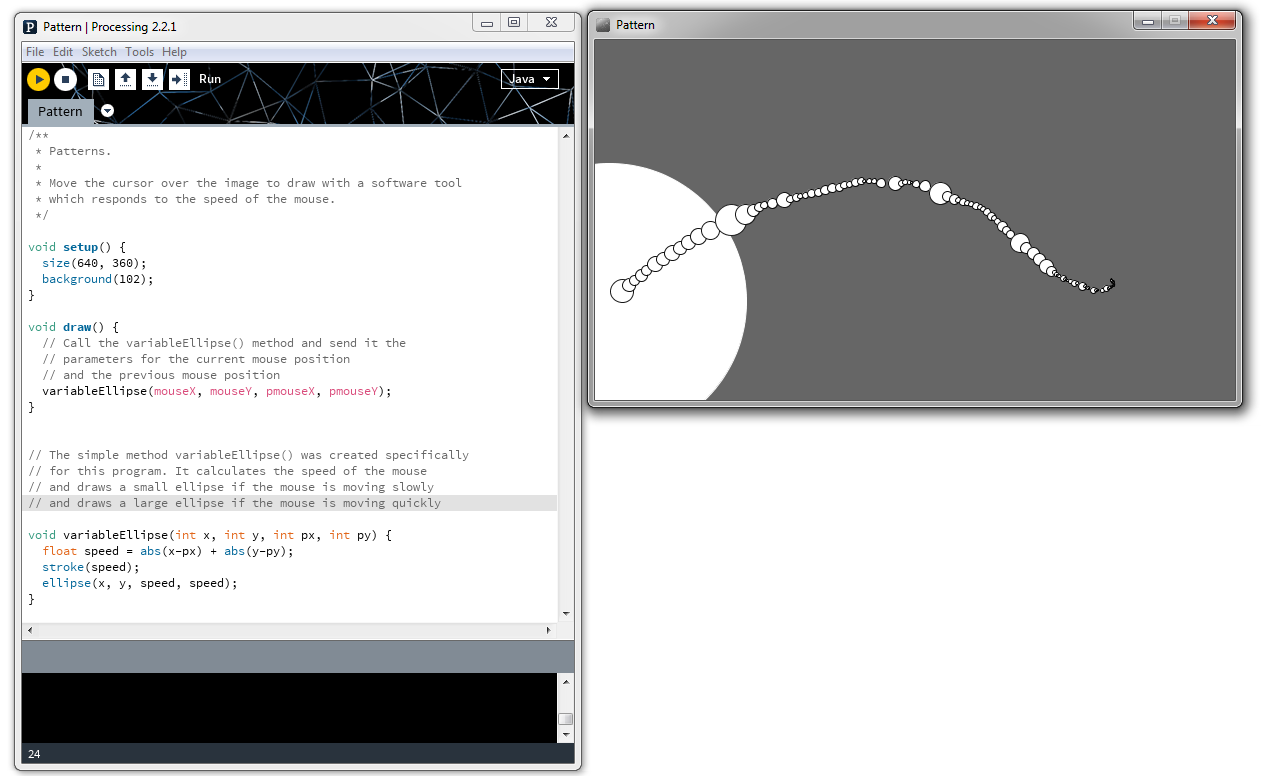
\includegraphics[width=1.0\textwidth]{images/proc_dev_env}
	\caption{On the left: The \gls{pde} displaying an example \emph{sketch} while it is being run. On the right: The drawing window to which the \emph{sketch's} instructions are applied.}
	\label{fig:proc:dev:env}
\end{figure}


\subsection{DesignScript}
\label{section:designscript:related}
DesignScript\cite{aish2012designscript} is a programming language that was designed to suit the needs of architecture related design.

%DesignScript programming paradigms
DesignScript uses concepts from multiple programming paradigms like object-oriented, functional and associative programming.
Entities have properties that can be either data or functions like in object-oriented languages; functions' most important role is to take some input and produce some output without producing side-effects like in functional languages; and dependencies among variables are retained like in associative languages.

It supports both imperative (following instructions step-by-step) and associative (propagating changes in a dependency graph) control flows.
The programmer can choose to have portions of the code following one type of control flow and other portions following the other.

%DesignScript primitives
Being a domain-specific language for architecture, DesignScript provides functions for 3D modeling such as creating concrete 3D objects, like cubes and spheres, as well as abstract geometry, like planes and points, that used as scaffolding.

DesignScript also supports lists of values and lets them be used in place of single parameters in calls to functions.
This lets architects use lists more easily as they do not have to use loops to extract values and the function.%
\footnote{If only one of its parameters is receiving a list instead of a value, the function is called once with each value on the list.
If more than one parameter is receiving a list, the function is called with the values combined by either a cross product or a zip of the lists.}

Having modeling primitives and combining several programming paradigms allows the architect to draw from knowledge about architecture modeling while empowering him to express the processes in which those primitives are used.

%DesignScript editor(s)
Editing DesignScript programs can be done either by writing or by creating a graph.
The graph is a more natural representation of the dependencies between the variables of the program when the associative paradigm is being used; it can also be viewed as a data-flow graph.
The written representation of DesignScript is a sequence of statements that specify the relationship between a variable and other variables; defining functions, using the imperative paradigm and reassigning variables is also possible.

DesignScript is used in several environments.
These include a textual editor in Autodesk AutoCAD (Fig. \ref{fig:ds:autocad}), a dedicated graph editor called DesignScript Studio (Fig. \ref{fig:ds:dsstudio}) and later Dynamo (Fig. \ref{fig:ds:dynamo}).
Both DesignScript Studio and Dynamo use graph based program editing.

\begin{figure}
	\centering
	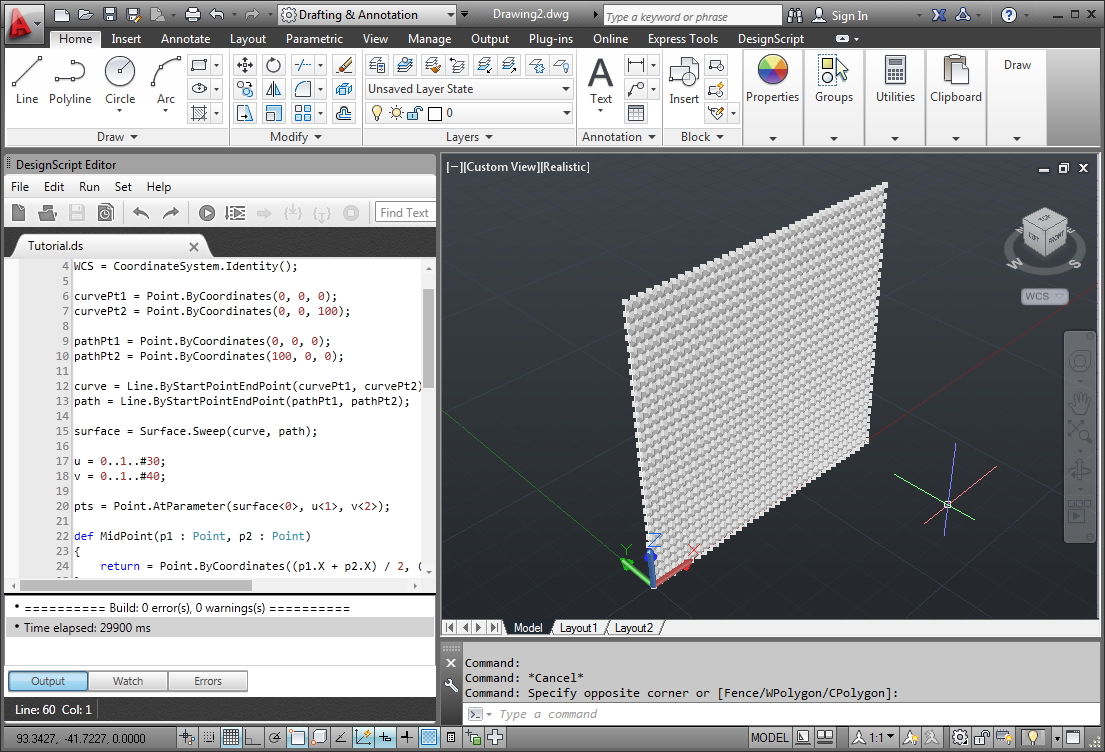
\includegraphics[width=0.8\textwidth]{images/ds_autocad}
	\caption{A DesignScript program being edited in a special text editor inside AutoCAD. This text editor provides auto-complete and a debugger.}
	\label{fig:ds:autocad}
\end{figure}

\begin{figure}
	\centering
	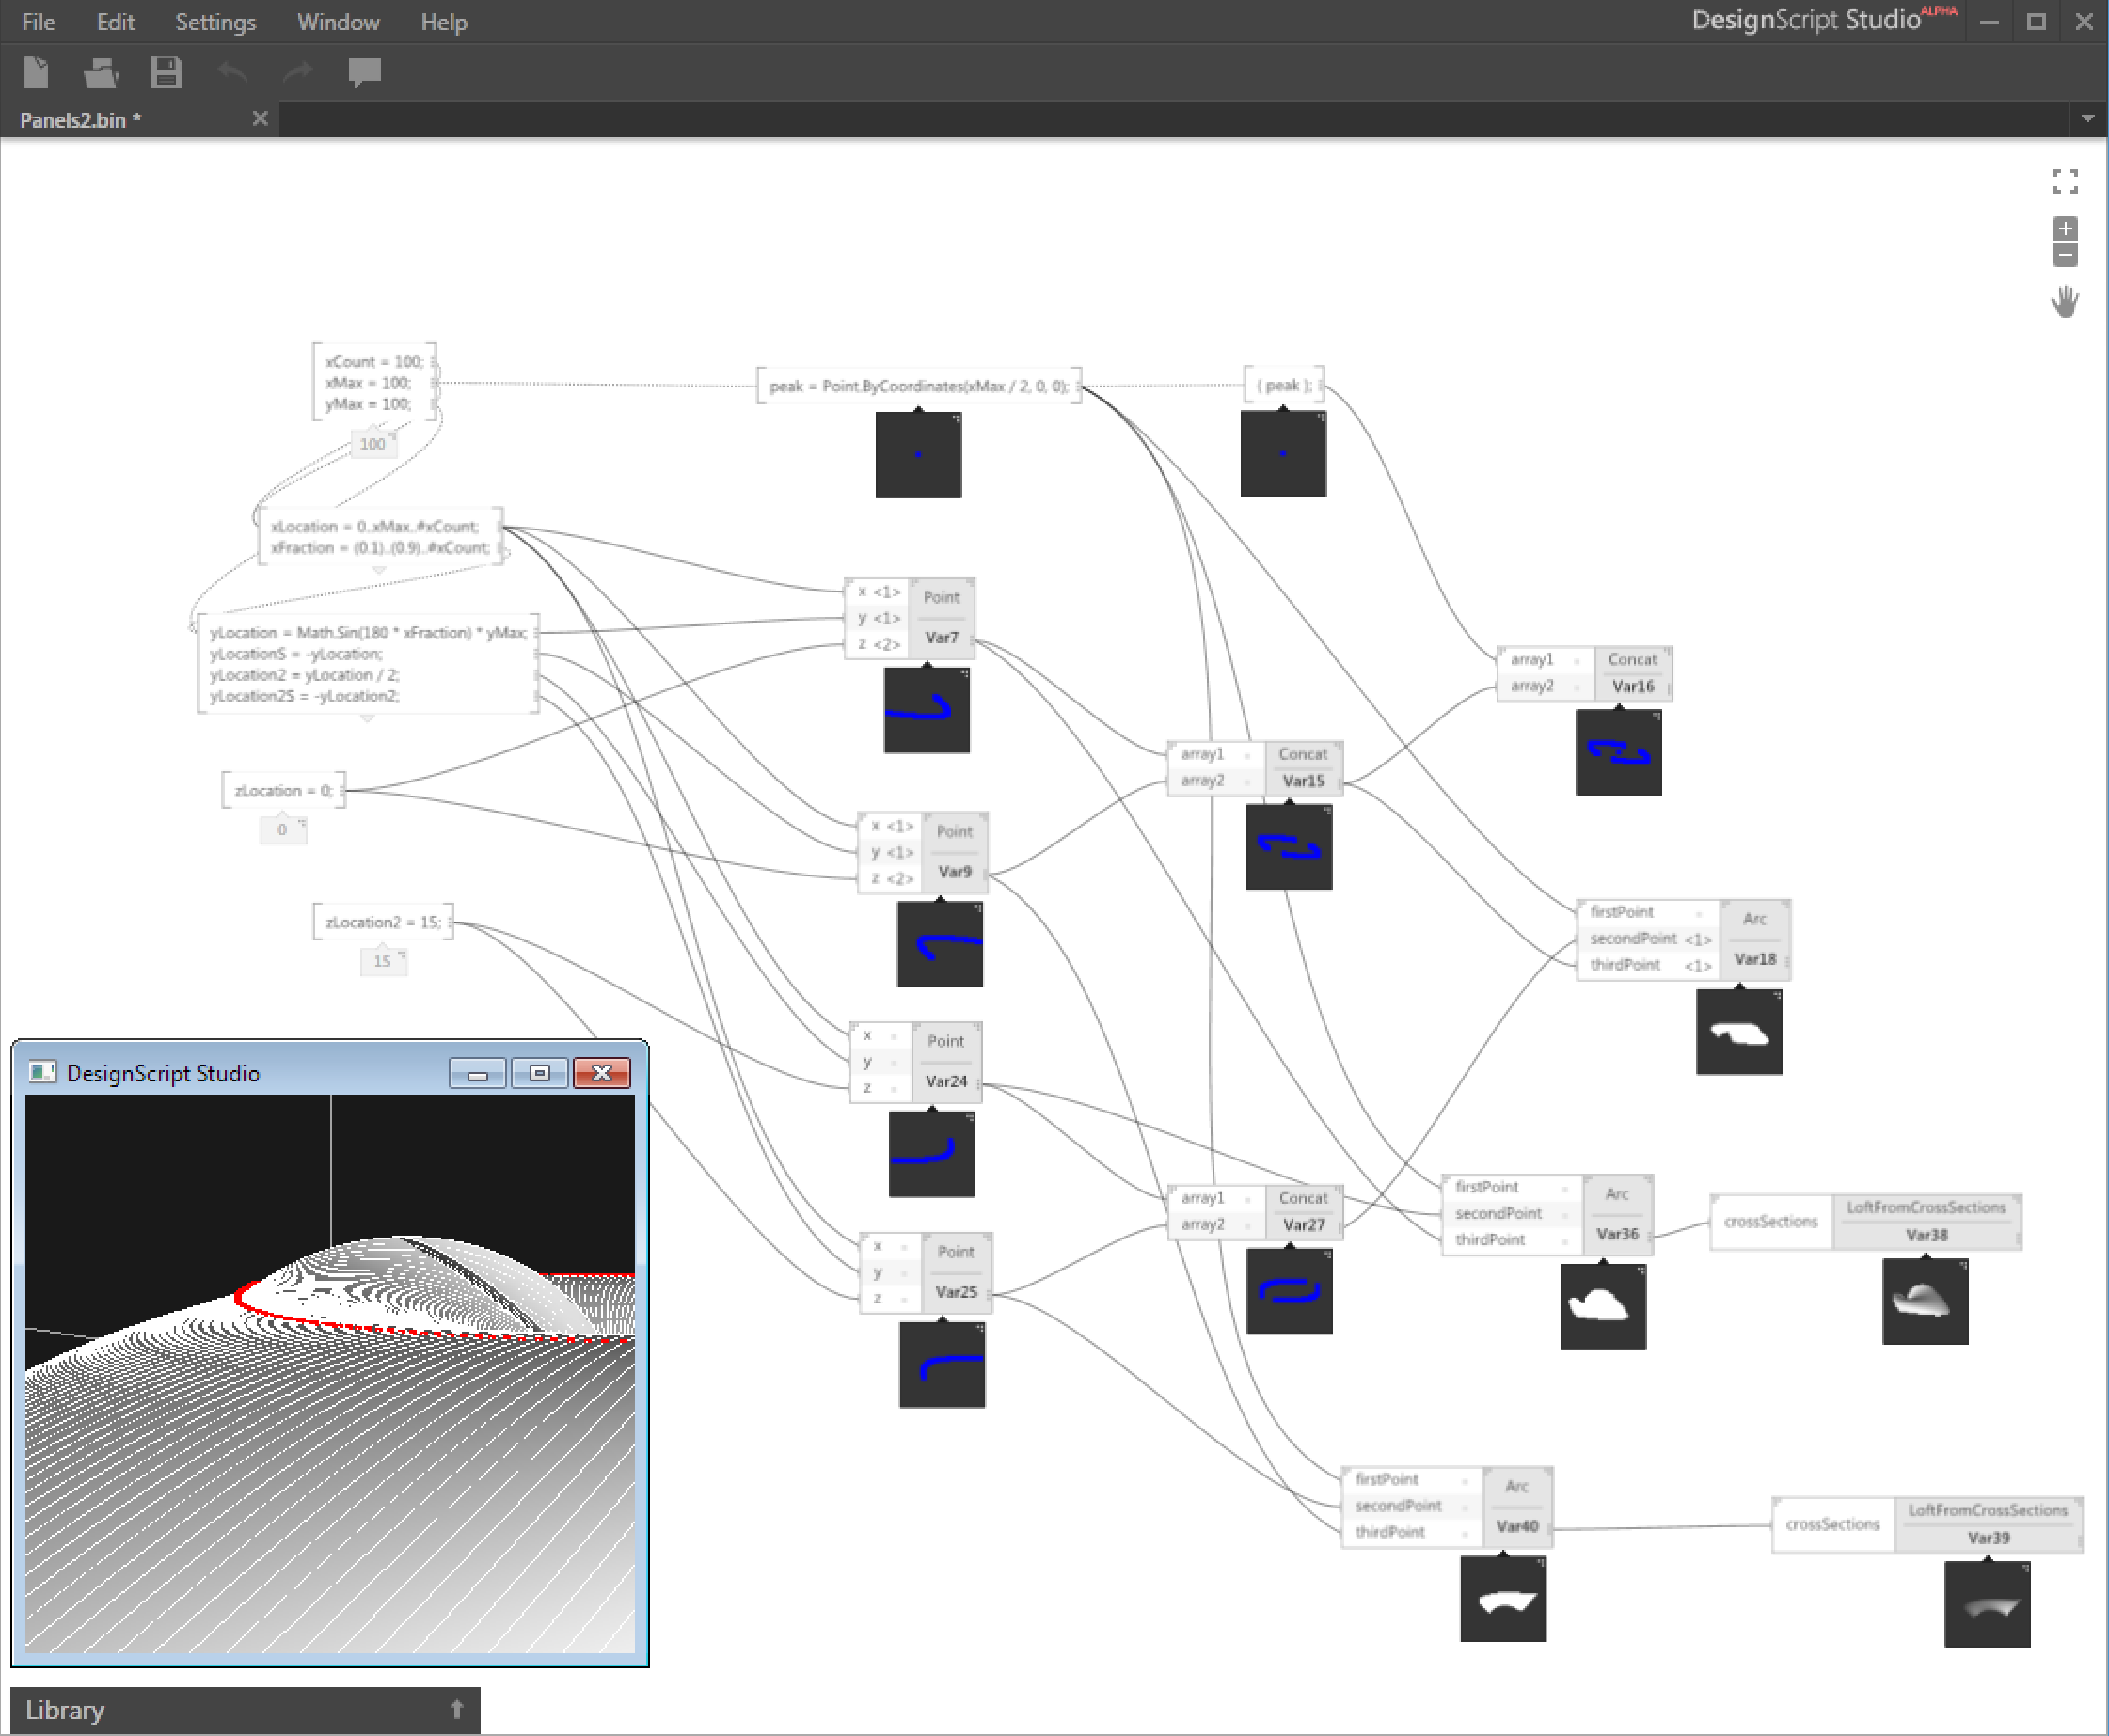
\includegraphics[width=0.8\textwidth]{images/ds_dsstudio}
	\caption{A DesignScript program as a graph in DesignScript Studio. Each node can display a preview of its results. To the bottom left corner is a preview of the whole program results and a folded library tab. The library tab contains everything that can be used in the program.}
	\label{fig:ds:dsstudio}
\end{figure}

\begin{figure}
	\centering
	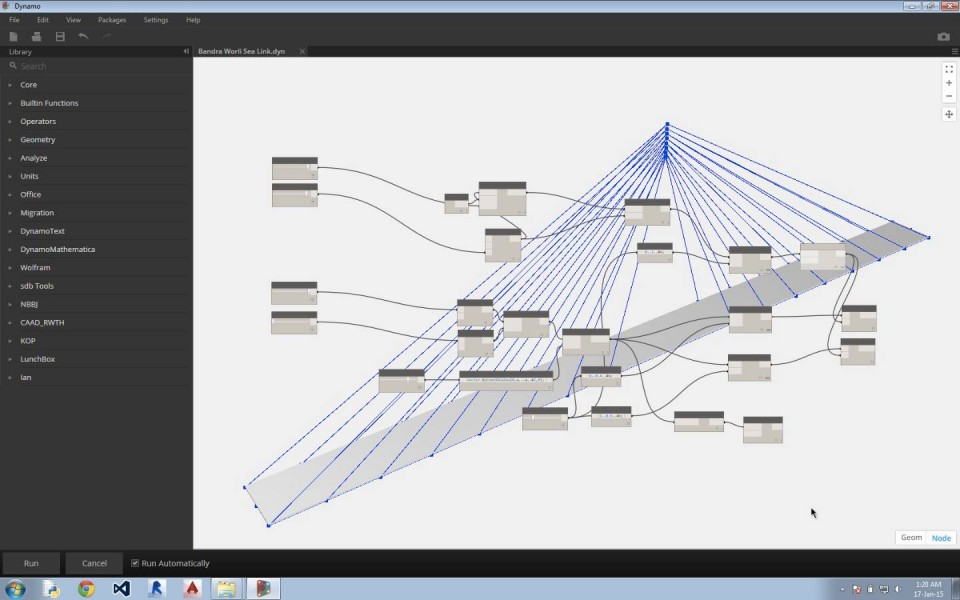
\includegraphics[width=0.8\textwidth]{images/ds_dynamo}
	\caption{Another DesignScript program as a graph in Dynamo. Like in DesignScript Studio, a preview of the result of the program is displayed. A difference is that there is only one preview ``canvas''; the preview from selected nodes is highlighted.}
	\label{fig:ds:dynamo}
\end{figure}

Debugging DesignScript programs depends on the environment being used.
The textual environment allows to follow the execution of the program step-by-step while also supporting watches and breakpoints.
The graph-based environments allow highlighting and listing results of each node.
Both the textual and the graph-based environments provide a preview of the execution of programs.

%DesignScript history
DesignScript was later used as the scripting language of Dynamo, integrated with Autodesk Revit, where programs are edited as data-flow graphs.
DesignScript was also integrated into Autodesk AutoCAD.
A standalone node-based DesignScript editor was also made, it was called DesignScript Studio.


\subsection{Rosetta}
\label{section:rosetta:related}
Rosetta\cite{de2012modern,lopes2011portable}, shown in Fig. \ref{fig:rosetta:ex}, is a platform for \gls{gd}.

Most CADs architects use allow them to make \gls{gd} program.
The problem with programming is that as each of these CADs has specific primitive operations, so, programs written for one CAD will only work in that CAD.
As an example, if one writes a program for AutoCAD, he cannot use it in Rhinoceros3D.
He really wants to use it in Rhinoceros3D, he has to rewrite it taking into account the differences between primitive operations of both \glspl{cad}.

Rosetta's motivation is to allow architects to write portable \gls{gd} programs that generate equivalent models in the CADs they use.

Rosetta does this by allowing the architect to choose the front-end programming language and the back-end where the primitive operations will be performed.\footnote{Some front-ends supported by Rosetta are AutoLisp (one of AutoCAD's programming languages), Javascript, Racket and Python; some of the supported back-ends include CADs like Autodesk AutoCAD, Autodesk Revit, Sketchup, and Rhinoceros 3D and also graphics libraries like TikZ and OpenGL.}
This way, the architect can experiment with \gls{gd} without having to switch \gls{cad} and he can also share programs with others using different \glspl{cad}.

Rosetta also allows programs written in one programming language to use not only parts from programs written in the same language, but also from programs written in other languages.
This eliminates the need to use the same programming language throughout a program and enables the use of programs written in any programming languages.

\begin{figure}
	\centering
	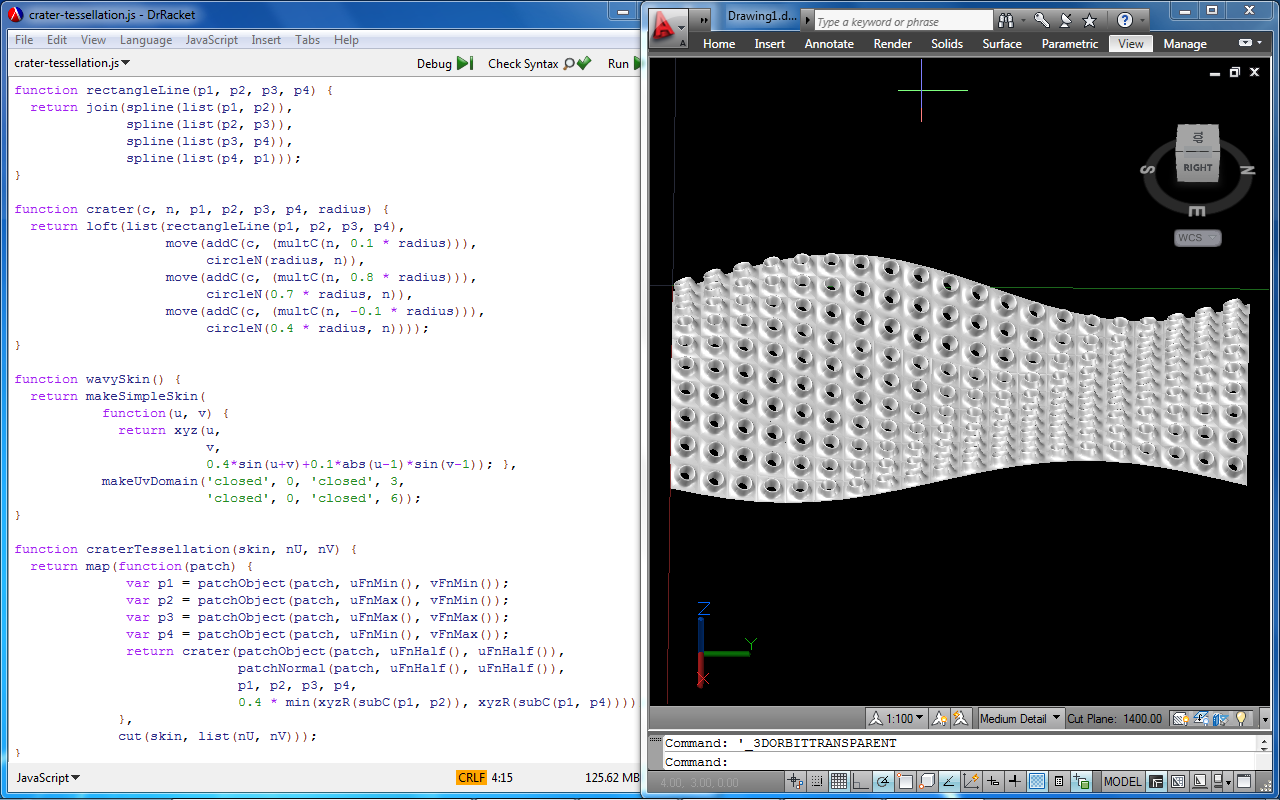
\includegraphics[width=0.8\textwidth]{images/rosetta_js_autocad}
	\caption{A Rosetta program (left) and AutoCAD displaying its results (right). The program is written in Javascript.}
	\label{fig:rosetta:ex}
\end{figure}


%##############################################################################
%##############################################################################
\section{Problems to Address}
